\section{Results}

\subsection{Main Result: INT2 Is the Regime Where Correction Matters}

Figure~\ref{fig:int2_curve} shows the strongest result in the project: near-IID
CIFAR-10 with INT2 quantization and only 20\% anchors. This is the regime where
plain averaging struggles most because each uploaded coordinate has only three
effective levels.

\begin{figure}[h]
  \centering
  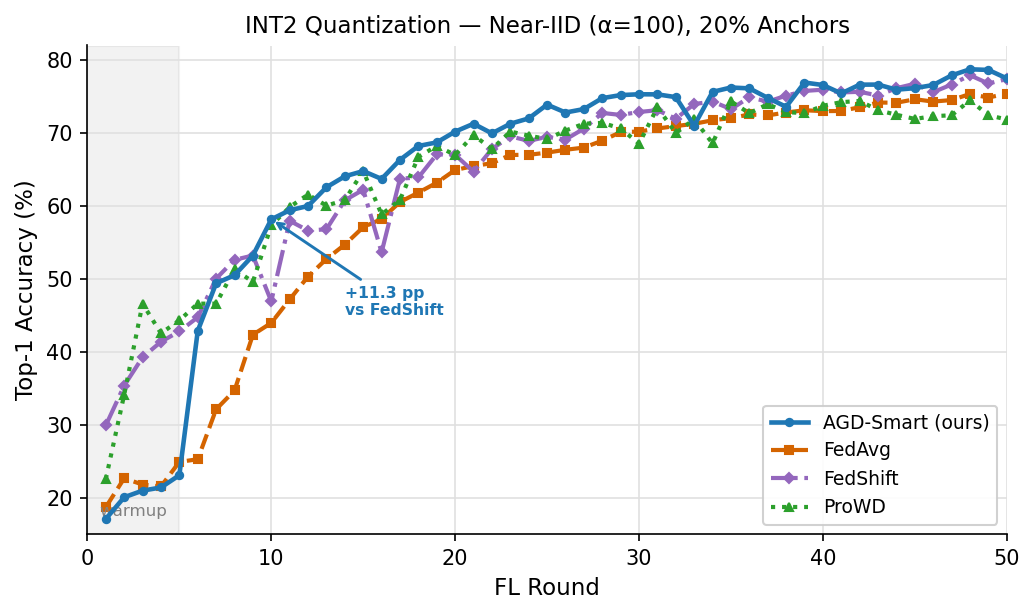
\includegraphics[width=\columnwidth]{int2_curve.png}
  \caption{INT2 near-IID benchmark over 50 rounds. \method gains sharply after
  warmup and stays ahead of FedAvg throughout the full run.}
  \label{fig:int2_curve}
\end{figure}

\begin{table}[h]
  \centering
  \caption{INT2 near-IID checkpoints (\%).}
  \label{tab:int2_checkpoints}
  \begingroup
  \footnotesize
  \setlength{\tabcolsep}{5pt}
  \begin{tabular}{lcccc}
    \toprule
    Method & R10 & R20 & R30 & R50 \\
    \midrule
    FedAvg                    & 44.0 & 64.9 & 70.2 & 75.4 \\
    FedShift                  & 46.9 & 67.0 & 72.9 & 77.4 \\
    ProWD                     & 57.3 & 67.0 & 68.5 & 71.8 \\
    \textbf{\method}          & \textbf{58.2} & \textbf{70.2} & \textbf{75.3} & \textbf{77.5} \\
    \bottomrule
  \end{tabular}
  \endgroup
\end{table}

Table~\ref{tab:int2_checkpoints} shows that \method is the best method at every
reported checkpoint, but the comparison to FedShift changes the interpretation
of the result. FedShift already fixes much of the end-of-training bias: by
round 50 it reaches 77.4, essentially tied with \method at 77.5 and clearly
above FedAvg. The remaining advantage of \method is therefore front-loaded. It
leads FedShift by +11.3 points at round 10 and by +3.2 at round 20, which is
exactly the interval where a communication-limited system benefits most from a
stronger correction policy. Relative to ProWD, the gap still widens over time,
reaching +5.7 at round 50. That separates the three correction strategies
clearly: ProWD forgets too much from round to round, FedShift eventually
recovers but reacts slowly, and \method combines fast activation with strong
final accuracy.

\subsection{Noise Scaling}

Table~\ref{tab:noise_scaling} shows that the method's value is highly dependent
on quantization severity. Once the bit-width rises to INT3 or above, FedAvg is
usually good enough. The correction pipeline becomes most valuable when the
quantized representation collapses too much directional information. FedShift
was rerun only on the four shared headline configurations, so this table keeps
the broader bit-width threshold comparison against FedAvg and ProWD.

\begin{table}[h]
  \centering
  \caption{Round-20 accuracy under different near-IID bit-widths with 20\%
  anchors.}
  \label{tab:noise_scaling}
  \small
  \resizebox{0.95\columnwidth}{!}{%
  \begin{tabular}{lccccc}
    \toprule
    Bits & Levels & FedAvg & ProWD & \method & vs. FedAvg \\
    \midrule
    INT8 & 255 & 72.0 & 66.4 & 68.2 & $-3.9$ \\
    INT6 & 63  & 73.0 & 68.3 & 70.7 & $-2.2$ \\
    INT4 & 15  & 74.5 & 65.4 & 72.8 & $-1.7$ \\
    INT3 & 7   & 74.4 & 65.8 & 71.7 & $-2.8$ \\
    INT2 & 3   & 65.4 & 59.8 & \textbf{70.7} & \textbf{+5.3} \\
    \bottomrule
  \end{tabular}}
\end{table}

Table~\ref{tab:noise_scaling} makes the crossover point very clear. Compared
with ProWD, \method wins at every bit-width, from +1.8 points at INT8 up to
+10.9 points at INT2, so the improved correction design is consistently better
than the simpler learned baseline. Compared with FedAvg, however, the sign of
the gain flips with quantization severity: \method is still 1.7--3.9 points
behind from INT8 through INT3, then jumps to a +5.3 advantage at INT2. That
pattern supports the main claim of the paper. Learned dequantization is not
universally necessary, but it becomes valuable once the quantizer is coarse
enough that plain averaging cannot preserve update direction. The shared
FedShift reruns follow the same story: it is competitive in the easier near-IID
settings and helpful at INT2, but the learned model becomes more valuable once
early convergence or heterogeneous matching matters.

\subsection{Behavior in Milder Regimes}

Figure~\ref{fig:other_curves} summarizes the remaining reported settings. The
pattern is consistent: \method reliably beats ProWD, but it only surpasses
FedAvg once quantization is severe enough that averaging alone can no longer
recover the signal.

\begin{figure*}[t]
  \centering
  \begin{subfigure}{0.32\textwidth}
    \centering
    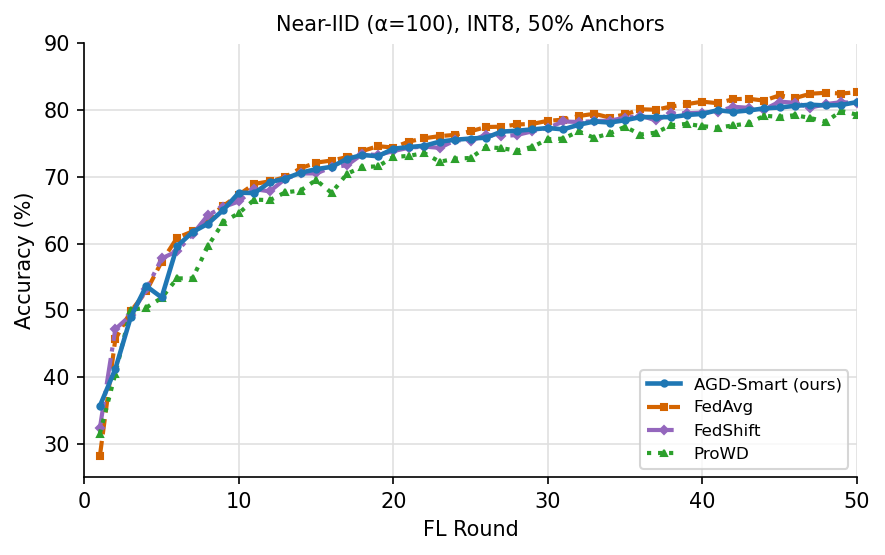
\includegraphics[width=\linewidth]{int8_curve.png}
    \caption{Near-IID, INT8}
  \end{subfigure}\hfill
  \begin{subfigure}{0.32\textwidth}
    \centering
    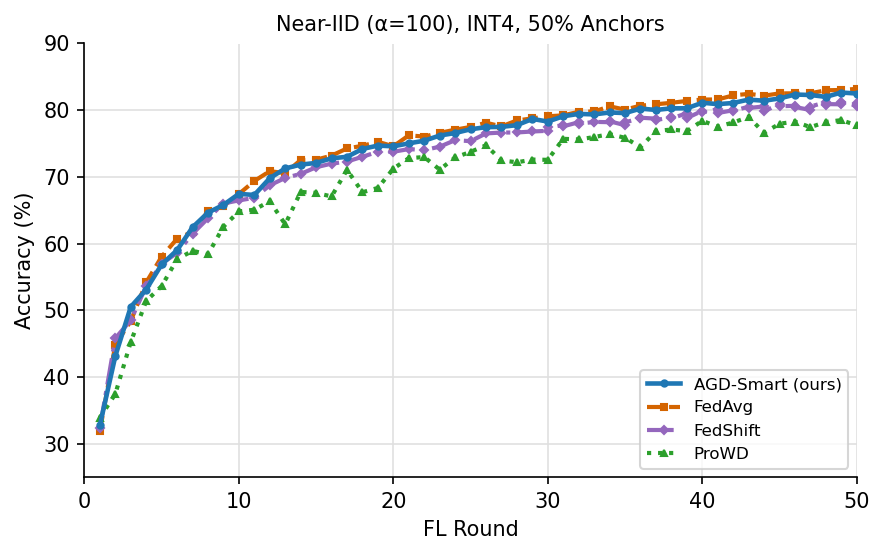
\includegraphics[width=\linewidth]{int4_curve.png}
    \caption{Near-IID, INT4}
  \end{subfigure}\hfill
  \begin{subfigure}{0.32\textwidth}
    \centering
    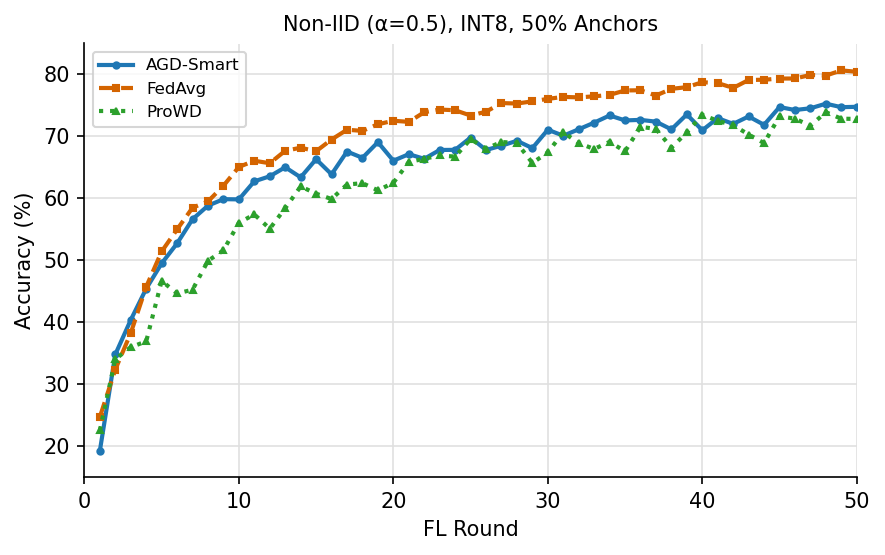
\includegraphics[width=\linewidth]{noniid_curve.png}
    \caption{Non-IID, INT8}
  \end{subfigure}
  \caption{Secondary regimes. The method stays consistently above ProWD, nearly
  matches FedAvg under near-IID INT4, and narrows the gap to FedAvg under
  non-IID INT8 without fully closing it.}
  \label{fig:other_curves}
\end{figure*}

\begin{table*}[t]
  \centering
  \caption{Summary across shared configurations, including FedShift.}
  \label{tab:summary}
  \small
  \resizebox{0.95\textwidth}{!}{%
  \begin{tabular}{lccccc}
    \toprule
    Setting & FedShift @ R50 & \method @ R50 & vs. FedShift & vs. ProWD & vs. FedAvg \\
    \midrule
    Near-IID, INT2, 20\% anchors & 77.4 & 77.5 & +0.1 & +5.7 & +2.1 \\
    Near-IID, INT8, 50\% anchors & 81.1 & 81.2 & +0.1 & +1.9 & -1.5 \\
    Near-IID, INT4, 50\% anchors & 80.7 & 82.5 & +1.8 & +4.8 & -0.7 \\
    Non-IID, INT8, 50\% anchors  & 73.8 & 74.8 & +1.0 & +2.0 & -5.6 \\
    \bottomrule
  \end{tabular}}
\end{table*}

Table~\ref{tab:summary} sharpens the baseline story. FedShift is the stronger
lightweight comparator: it beats ProWD in three of the four shared settings and
nearly matches \method at the easier near-IID endpoints. That makes the INT4
and non-IID rows more informative than the near-IID INT8 tie. At INT4,
\method keeps a +1.8 final advantage over FedShift while finishing within 0.7
of FedAvg. Under non-IID INT8, the final gap is +1.0 and the midpoint gap is
+3.9 at round 25, which suggests that smart client-to-anchor matching matters
more than a single global shift once anchor and constrained populations no
longer share the same mean direction. INT2 is different again: the final
accuracy is nearly tied, but the route to that endpoint is not.

\begin{figure}[t]
  \centering
  \resizebox{0.98\columnwidth}{!}{\begin{tikzpicture}[x=0.62cm,y=0.82cm,font=\small]
  \def\barhalf{0.17}

  \node[anchor=west,font=\bfseries] at (0,4.9) {Round 10 gain over FedShift};
  \node[anchor=west,font=\bfseries] at (14,4.9) {Round 50 gain over FedShift};

  \foreach \x/\lab in {0/0,2/2,4/4,6/6,8/8,10/10,12/12} {
    \draw[gray!25] (\x,0.45) -- (\x,4.35);
    \node[font=\scriptsize] at (\x,0.08) {\lab};
  }
  \draw[->,thick] (0,0.45) -- (12.55,0.45);
  \node[font=\scriptsize] at (6.2,-0.28) {percentage points};

  \foreach \x/\lab in {14/0,15/0.5,16/1.0,17/1.5,18/2.0} {
    \draw[gray!25] (\x,0.45) -- (\x,4.35);
    \node[font=\scriptsize] at (\x,0.08) {\lab};
  }
  \draw[->,thick] (14,0.45) -- (18.55,0.45);
  \node[font=\scriptsize] at (16.25,-0.28) {percentage points};

  \foreach \y/\name/\early/\final in {
    4/{Near-IID INT2}/11.3/0.1,
    3/{Non-IID INT8}/2.0/1.0,
    2/{Near-IID INT4}/1.0/1.8,
    1/{Near-IID INT8}/1.3/0.1
  } {
    \node[anchor=east,align=right,text width=2.7cm] at (-0.25,\y) {\name};
    \fill[anchorblue!85] (0,\y-\barhalf) rectangle (\early,\y+\barhalf);
    \node[anchor=west,font=\scriptsize] at (\early+0.15,\y) {+\early};
    \pgfmathsetmacro{\finalx}{14 + 2*\final}
    \fill[buffergreen!85] (14,\y-\barhalf) rectangle (\finalx,\y+\barhalf);
    \node[anchor=west,font=\scriptsize] at (\finalx+0.12,\y) {+\final};
  }
\end{tikzpicture}
}
  \caption{\method's gain over FedShift at round 10 and round 50 on the four
  shared configurations. The largest early-round advantage appears under INT2,
  while the largest persistent end-of-training gain appears at INT4.}
  \label{fig:fedshift_gains}
\end{figure}

Figure~\ref{fig:fedshift_gains} makes that contrast explicit. FedShift is
already a very strong no-learning baseline when the client population is
near-IID. At near-IID INT8 and INT2, the final gap is only +0.1. But those
near ties hide where \method helps most. In the severe INT2 regime it opens an
11.3-point lead by round 10, which matters if communication rounds are scarce.
At INT4, it keeps a meaningful +1.8 end-of-training advantage, suggesting that
the replayed learned corrector is still buying something after simple mean
alignment has done its part. Under non-IID data, FedShift loses more clearly
because the anchor mean is no longer a reliable global target.
